\section{Gameplay}
Players roll two dice of their chosen colour at the start of their turn.
The values of these dice are not combined, but instead used to move two cubes around the board individually.

Players can score points by \textit{Pinching} (Section~\ref{sec:pinching}) the opponent's cubes by moving their own cube of equal numeric value on top of them, or by \textit{Bearing Off} (Section~\ref{sec:bearing-off}) their own cubes, by first forming a stack of like-valued cubes, and then moving them off the board.

\note The dice values cannot be combined unless the cubes are moved as a stack (see Section~\ref{sec:bearing-off})

\note At any point in the game, a player may choose to simply pass, doing nothing this turn\footnote{Passing is mentioned in the FAQ}.
The passing player \textbf{must} pass on both dice, and cannot simply move with one and pass on the other.

\note A player is permitted to simply move their cubes within the bank, though once they leave the bank, they cannot move back in unless as part of a set (see Section~\ref{sec:bearing-off}).

\subsection{Moving a Cube}
Before moving a cube, the cube must first be rotated to a different face.
This rotation is entirely based on whether the die rolled was even or odd.
After the cube has been rotated, it is then moved the indicated number of spaces orthogonally in any direction on the board, though never crossing back over the starting line.

Cubes also cannot pass over each other.

\paragraph{If the Die Shows Even} The cube's face value is increased to the next available value
$$1 \to 8 \to 16 \to 24 \to 32 \to 40 \to 1$$
\paragraph{If the Die Shows Odd} The cube's face value is decreased to the previous value
$$40 \to 32 \to 24 \to 16 \to 8 \to 1 \to 40$$

\note In either case, a roll-over happens if a player tries to increase or decrease past the highest or lowest value respectively.

\begin{figure}[!h]
    \centering
    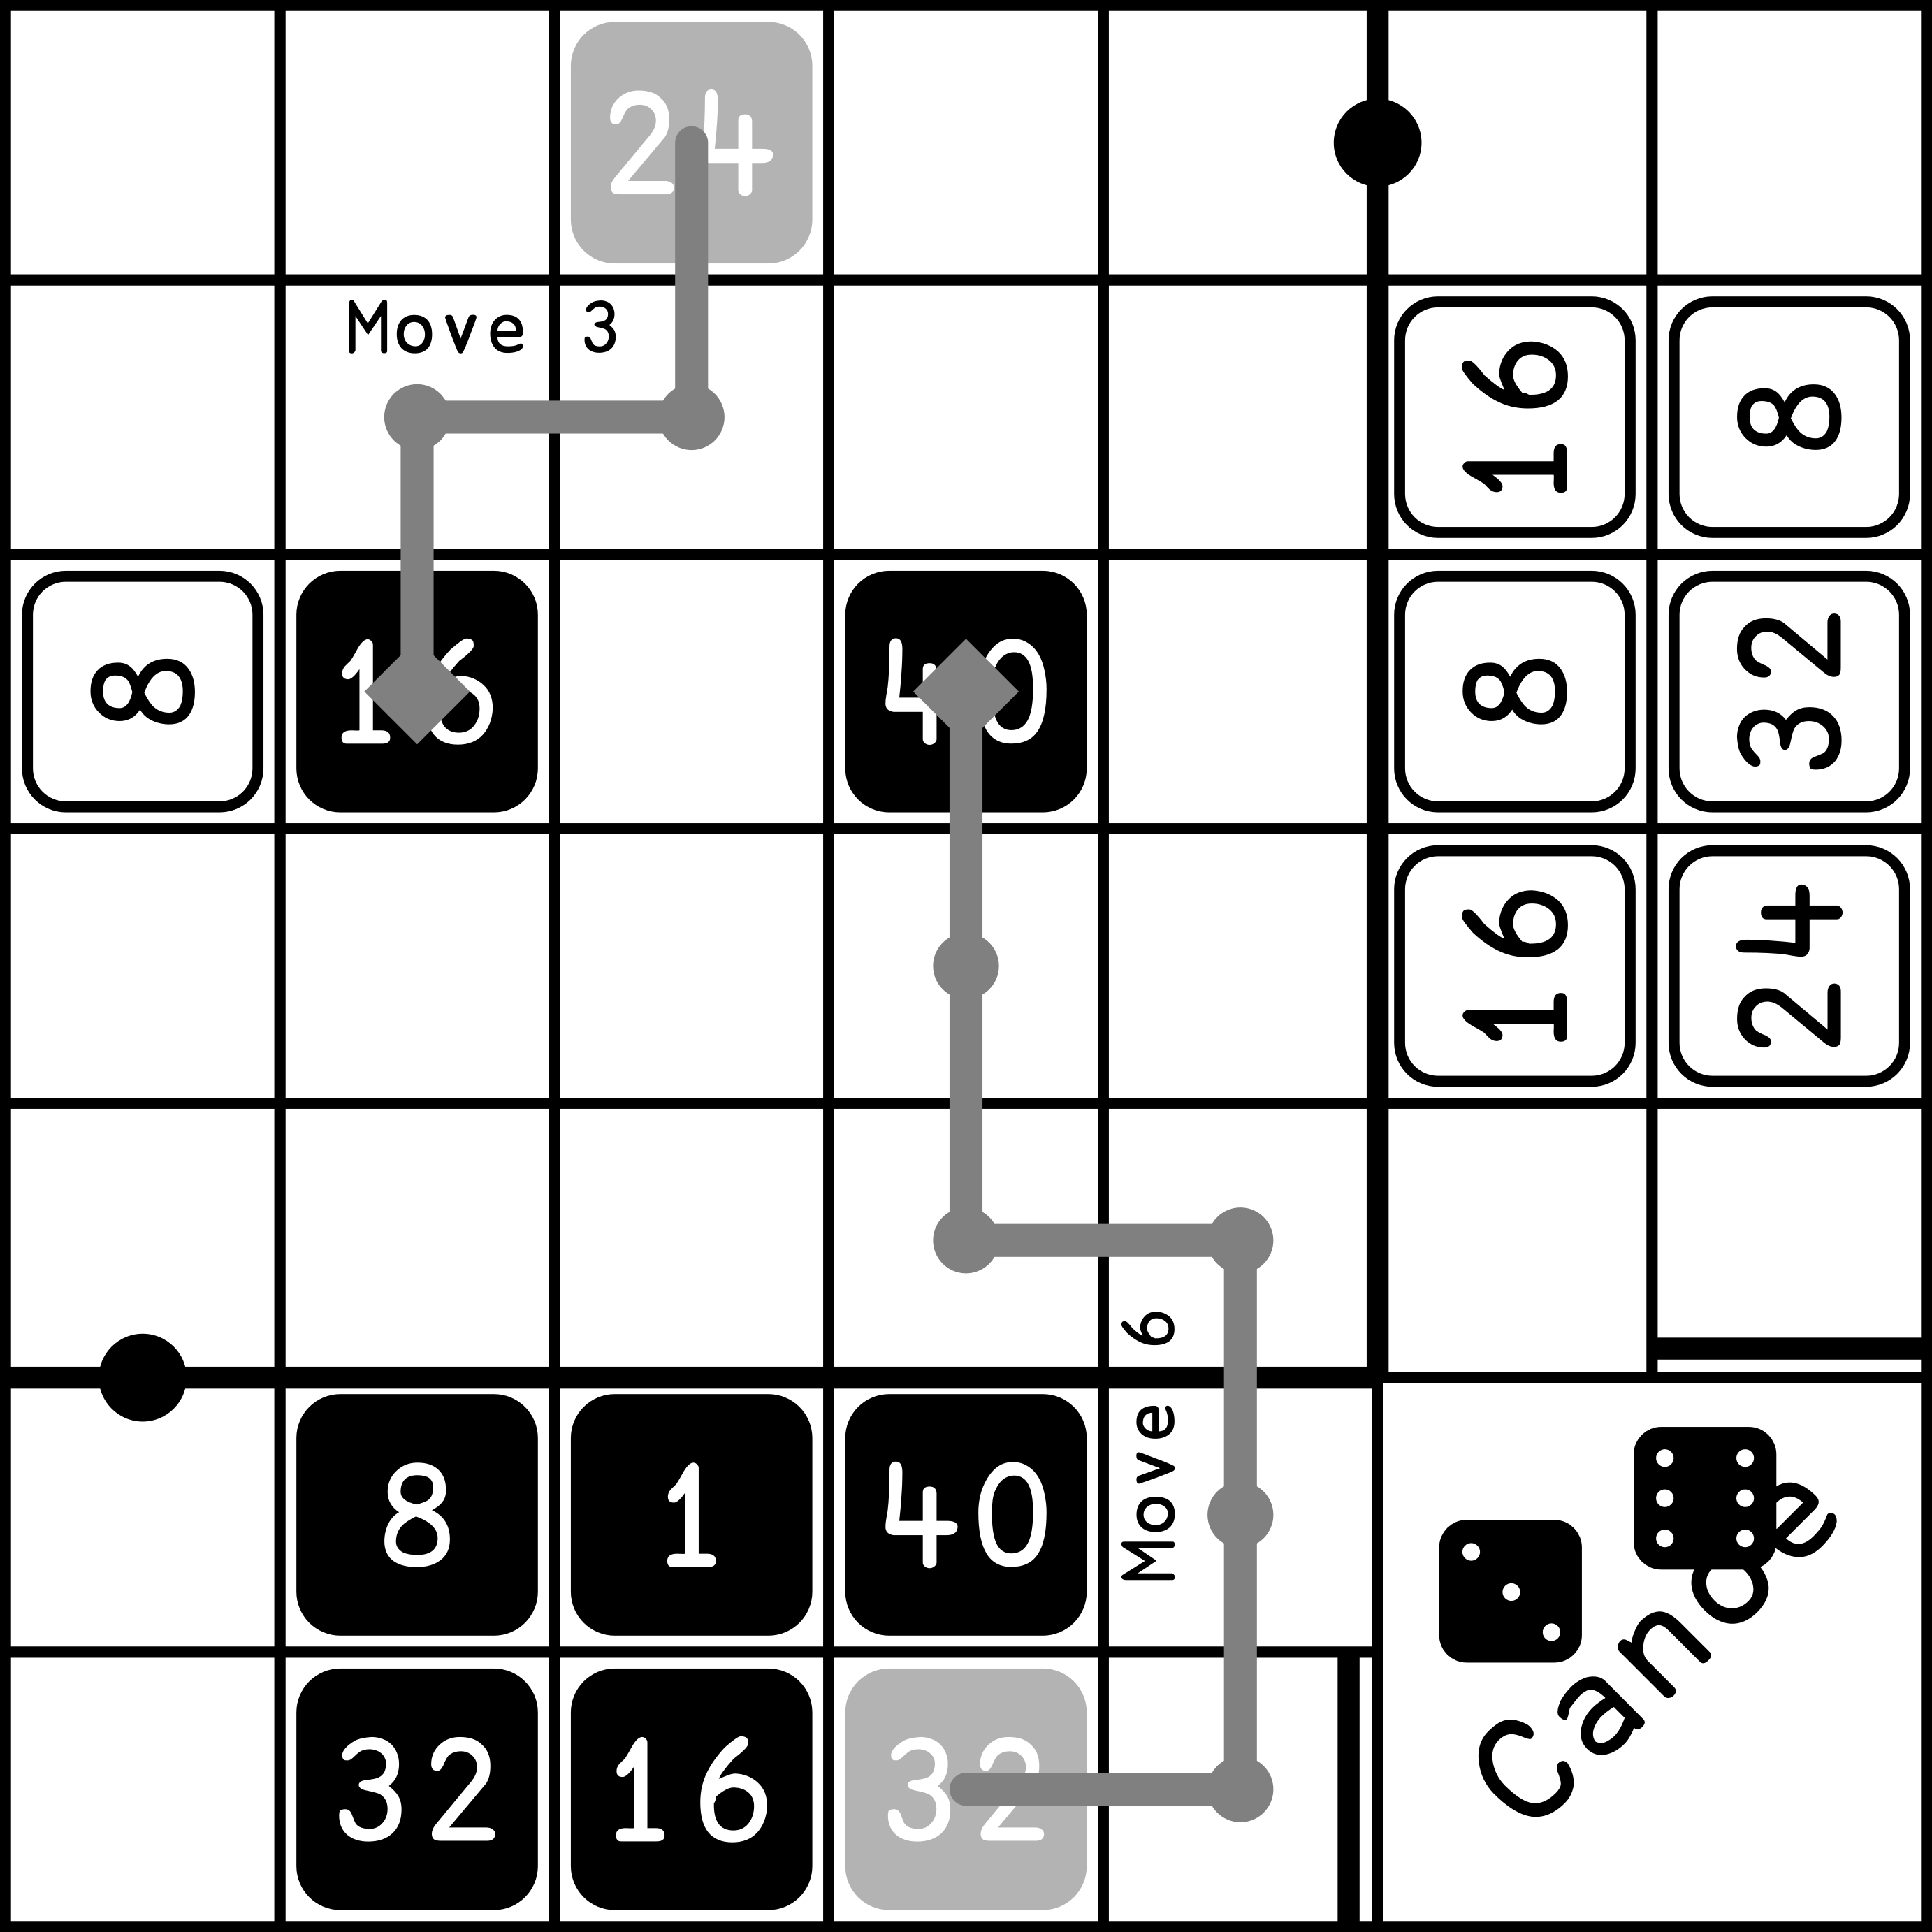
\includegraphics[width=8cm]{../graphics/movement}
    \caption{Example Move}
    \label{fig:move}
\end{figure}

\example In Figure~\ref{fig:move}, Billy rolled a \epsdice{6} and a \epsdice{3}, and has decided to move his 24 cube three spaces. 
He first rotates the cube so it shows 16 before moving it those three spaces. 
Next he wants to move his 32 cube six spaces, he first rotates the cube so it instead shows 40, and then moves it six spaces.

\subsubsection{Stymie}
In the event that a player has exactly two cubes left, and both share the same number and are either adjacent or have an even number of spaces between them, then that player may choose to call ``Stymie'' and only roll one die on their turn.
\subsection{Pinching}\label{sec:pinching}
Pinching is when a player moves their cube onto an opponent's cube of equal value.

Pinched cubes are removed from play and placed in the pincher's pocket.

\example Suppose Black has a 32 cube, and Ivory has a 24 cube four spaces away. 
Ivory rolls a four, and is now able to pinch Black's cube by first increasing the value up from 24 to 32, then moving the cube four spaces onto Black's cube.
Black's cube is removed from the game, scoring Ivory 32 points.

\paragraph{Note} It is not allowed on the first move by the first player.

\paragraph{Note} You cannot pinch with a cube that just crossed the starting line.
\subsection{Bearing Off}\label{sec:bearing-off}
To bear off, a player must first make a \textit{Set} by stacking two of their own cubes of like value, similar to Pinching.

Sets are special because they break the normal movement rules:
\begin{enumerate}
    \item Sets do not rotate before moving. If the cubes show 16, then they'll show 16 even after moving.
    \item Sets can jump over \textbf{any number} of adjacent other cubes or sets as part of their movement (see Figure~\ref{fig:jump}). This jump counts as just one move. Single cubes \textbf{cannot} jump.
    \item When moving sets you can \textit{add together} the results of both dice. This is not possible when moving cubes.
    \item Sets cannot pinch, only jump.
    \item Sets must move directly towards the pin on the board, and are not allowed to meander.
\end{enumerate}
\begin{figure}[!h]
    \centering
    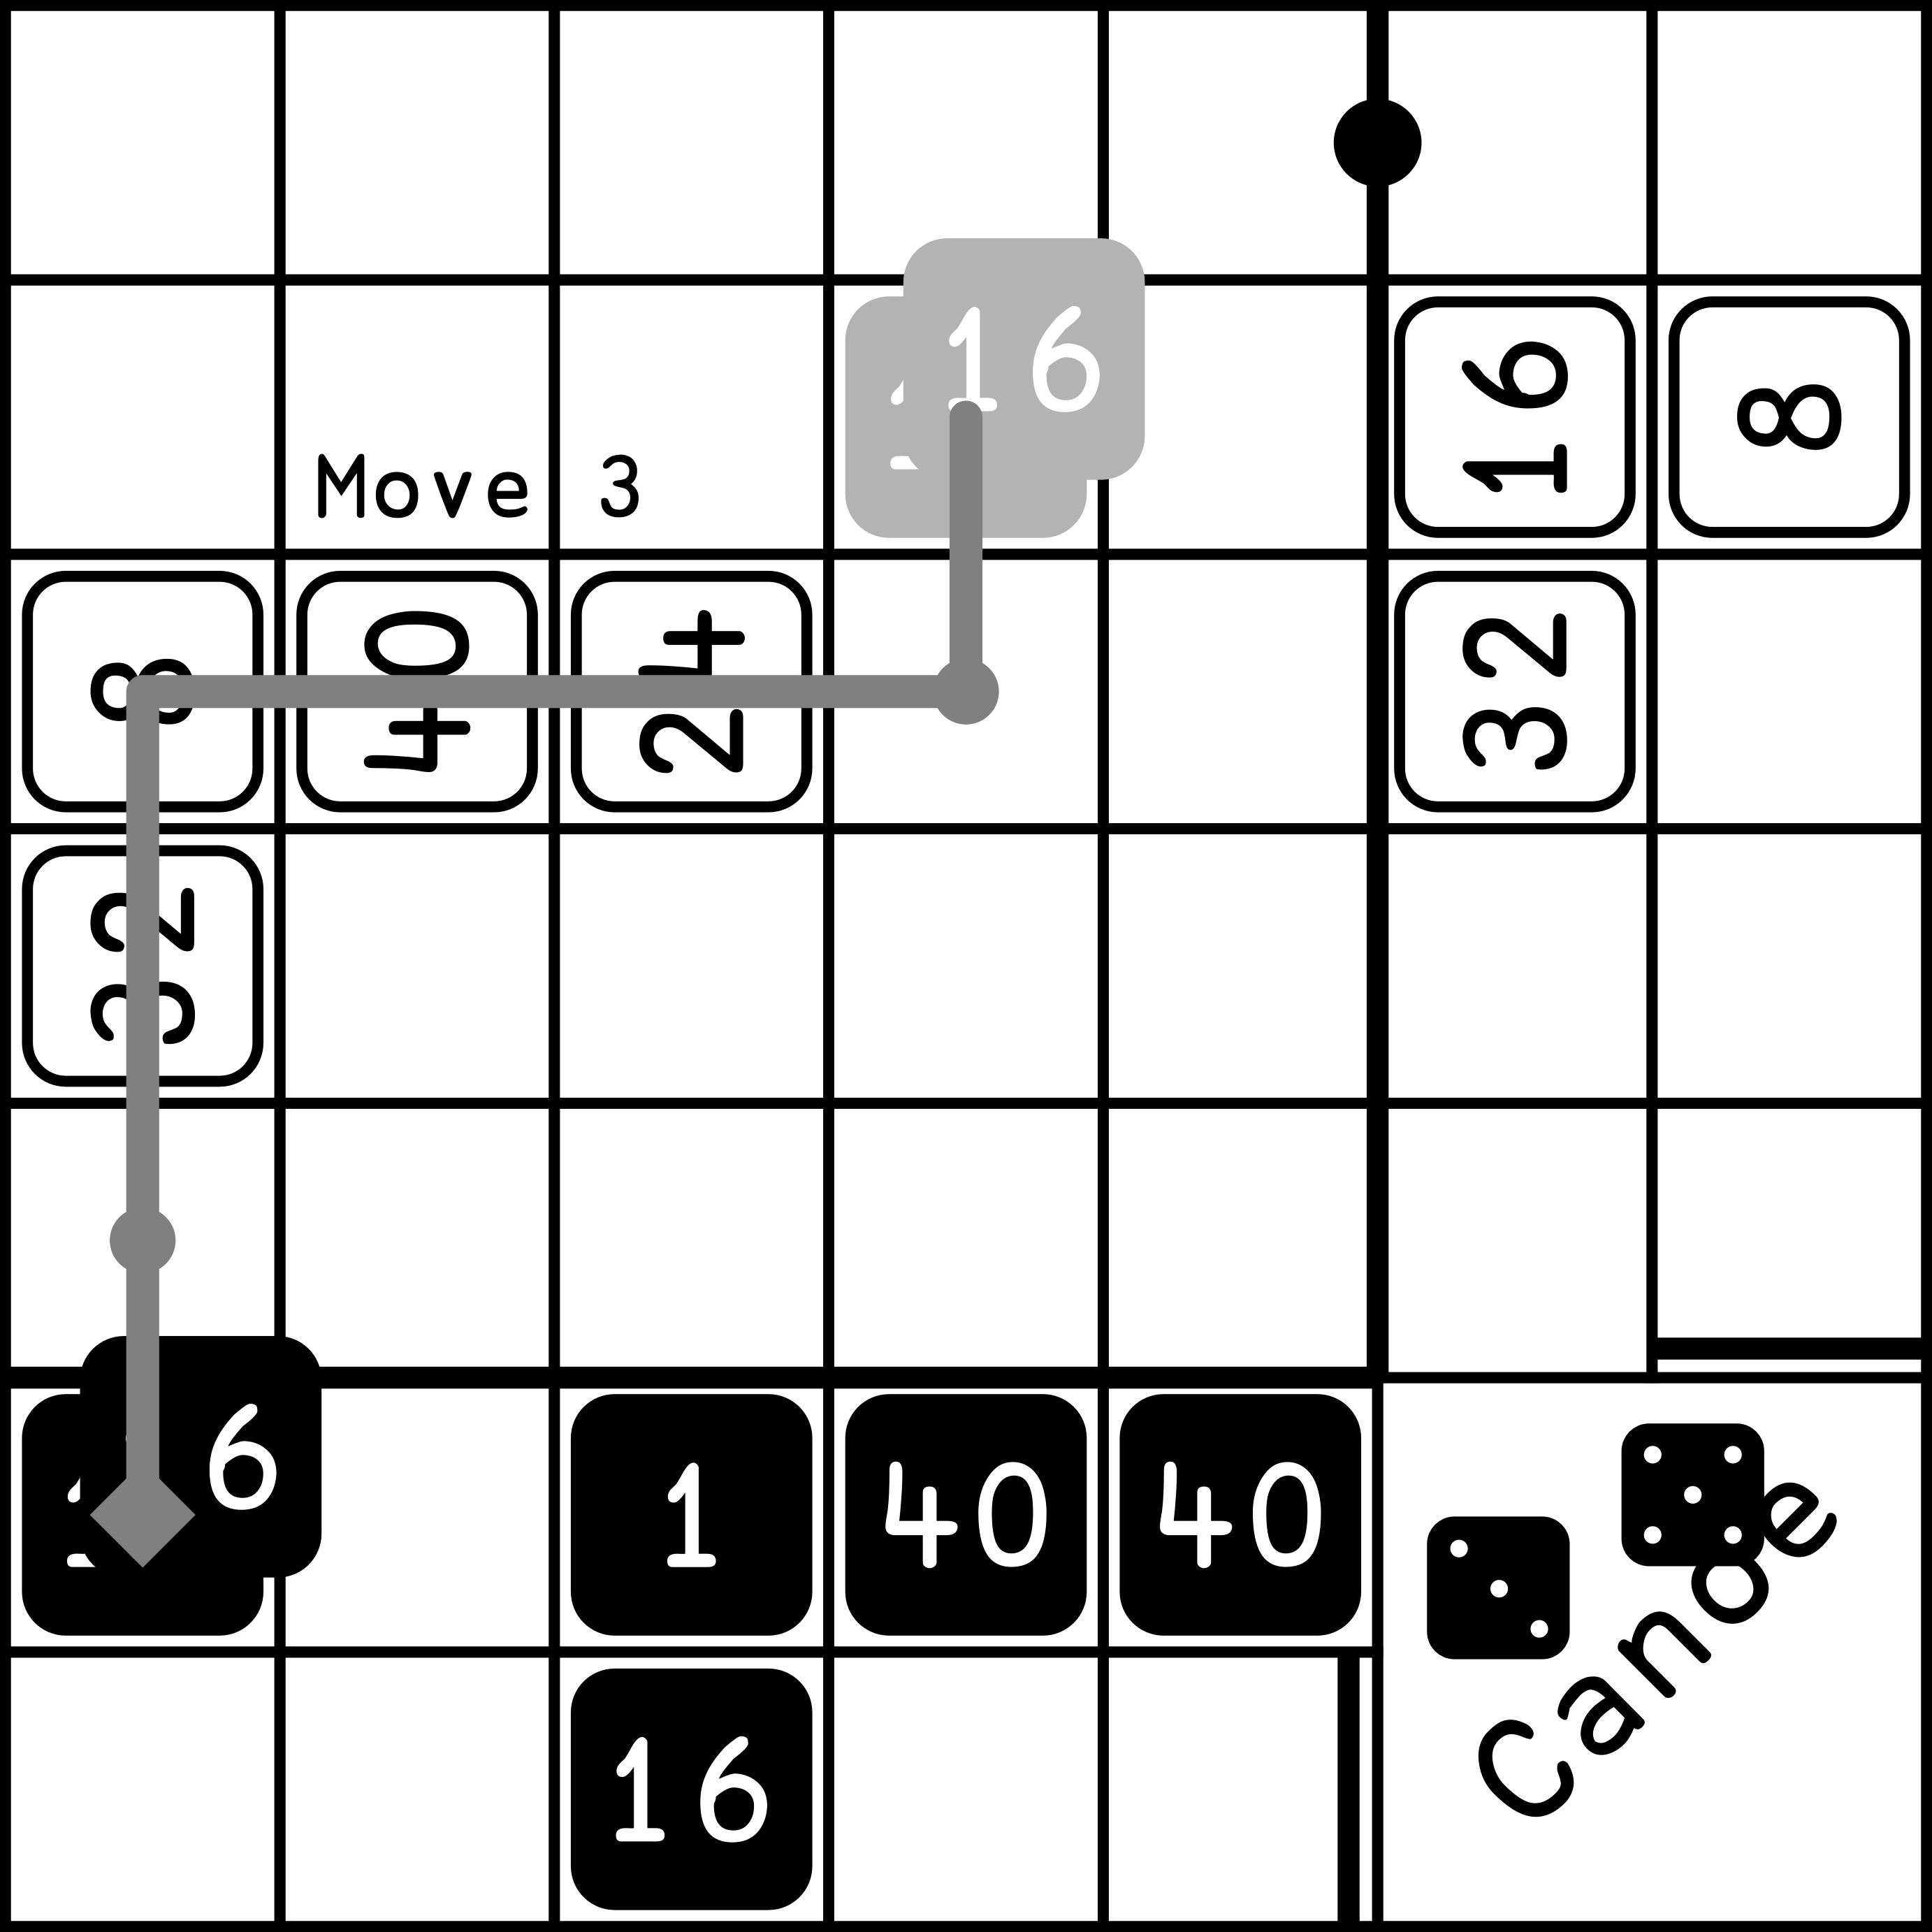
\includegraphics[width=8cm]{../graphics/jump}
    \caption{Example Jump}
    \label{fig:jump}
\end{figure}
To then bear off, a player must move the stack of cubes over the pin (black dot) on the starting line and into the bank, before then having to move towards the leather patch and over the line on the backmost row.

\paragraph{Jumping Example}
Figure~\ref{fig:jump} illustrates an example jump.
Black rolled a \epsdice{3} and a \epsdice{5}, and wishes to move their stack of 16s.
To get into the bank as quickly as possible, Black uses their \epsdice{3} and makes use of stacks' ability to jump over other pieces by first moving one down, then all the way over all of Ivory's pieces as the second move, only to end up inside the bank with a third move.

\paragraph{Note} You cannot make a set with a cube that's just left the bank.

\paragraph{Note} To bear off, a player needs the exact number or number combination to make it to the leather patch. If the roll isn't an exact match, it won't work.

\subsubsection{Canoe}
The first time a player bears off their cubes, \textit{both} of the cubes are pocketed for scoring.

All subsequent times, only one cube is pocketed, while the other is discarded, never to be seen again.

\subsubsection{Seventh Cube}
Once all but the last cube have been pinched or borne off, the seventh cube can then be borne off all by itself.
Doing so successfully sweeps the opponent's remaining cubes into the pocket as points.

Like a set, the seventh cube can also combine the results of the two dice for better reach.
Also like a set, the seventh cube must bear off as soon as possible.
\subsection{Sweeping}
Sweeping happens at the end of the game when bearing off your seventh and final cube.
Successfully doing so sweeps the board, giving you the other player's remaining cubes as points.

